\section{多重继承}
在上一章中,我们看到了C++流输入/输出库中复杂的继承关系。其中的 \lstinline@std::basic_iostream@ 尤为引人注目。你没看错,这个类同时继承自 \lstinline@std::basic_ostream@ 和 \lstinline@std::basic_istream@。这种继承多个基类的操作叫做\textbf{多重继承(Multiple Inheritance)}。\par
多重继承并不神秘。如果我们把继承视作是单纯的内嵌一个基类对象的话(私有继承是这样做的),那么多重继承就意味着在派生类对象中同时内嵌两个基类对象;如果我们把继承视作是共性成员的代码重用的话(公开继承是这样做的),那么多重继承就意味着派生类同时拥有这两个基类的特征。\par
以 \lstinline@std::stringstream@ 为例,它继承自 \lstinline@std::iostream@,而 \lstinline@std::iostream@ 多重继承自 \lstinline@std::istream@ 和 \lstinline@std::ostream@,所以它同时拥有 \lstinline@>>@ 和 \lstinline@<<@ 运算符的重载。于是这个类的对象既有输入功能又有输出功能。\par
\begin{lstlisting}
    std::stringstream ss;
    std::string str;
    ss << "1024"; //向ss对象中输出1024
    ss >> str; //把ss对象中的内容输入到str中
    std::cout << str; //用std::cout把str中的内容输出到屏幕上
\end{lstlisting}
这段代码演示了字符串输入/输出功能。\lstinline@std::stringstream@ 对象可以从字符串中读取输出,或者把自己读取到的内容输入到字符串中\footnote{我们规定,信息从输入设备、内存等处传递给程序叫做输入;从程序传递给输出设备、内存等处叫做输出。详见第十三章。}。\par
多重继承的语法也很简单,只要在继承列表中用逗号把若干基类隔开就行了。
\begin{lstlisting}
class A { /*...*/ };
class B { /*...*/ };
class Derived : public A, private B { /*...*/ }; 公开继承A,私有继承B
\end{lstlisting}\par
那么乍看上去,多重继承也没有什么特别的嘛,和单重继承差不多。其实不尽然,因为多重继承中有一些很麻烦的,我们不细想就想不到的问题。
\subsection*{多重继承中的名称歧义问题}
在单重继承时,是不会存在名称歧义的问题的。在单重继承时,如果我们在基类中定义了 \lstinline@id@ 而没有在派生类中定义 \lstinline@id@,那么使用派生类的成员 \lstinline@id@ 时,被使用的就是继承自基类的成员;如果我们在基类和派生类中都定义了 \lstinline@id@,那么使用用派生类的成员 \lstinline@id@ 时,被使用的就是派生类中定义的成员。如果我们非要使用基类的那个成员,就必须用显式地指定基类作用域,比如写成 \lstinline@Base::id@。\par
总之,单重继承中,无论如何,程序总是能为一个名称绑定到适当的函数上;即便因为多态而必须进行迟绑定,也不会存在因为歧义而不知绑定到哪个函数上的问题。\par
但在多重继承中,情况就变复杂了。我们完全可能遭遇这样的问题,两个基类中都有 \lstinline@id@ 这个名字,那么在进行多重继承时,这两个名字就会发生冲突。举个不太好的例子吧:我们要定义一个 \lstinline@Derived@ 类,它公开继承自 \lstinline@std::vector<int>@ 与 \lstinline@std::string@。
\begin{lstlisting}
class Derived : public std::vector<int>, public std::string {
    //公开继承自std::vector<int>,又公开继承自std::string
    Derived(const std::vector<int> &v, const std::string &s)
        : std::vector<int>{v}, std::string {s} {}
};
\end{lstlisting}
接下来,当我们要调用 \lstinline@length@ 成员函数时,编译器自然知道我们是要调用继承自 \lstinline@std::string@ 的 \lstinline@length@,因为 \lstinline@std::vector<int>@ 中并没有这个名称。
\begin{lstlisting}
    Derived d {{1,2,3,4},"str"};
    std::cout << d.length(); //编译器自然知道要调用的是什么;其返回值为3
\end{lstlisting}
但是当我们试图调用 \lstinline@size@ 成员函数时,问题出现了:
\begin{lstlisting}
    std::cout << d.size();
//error: request for member 'size' is ambiguous
\end{lstlisting}
出现这个问题的原因在于,\lstinline@Derived@ 从两个基类中各自继承了一个 \lstinline@size@ 成员函数。这两个成员函数之间没有覆盖关系,它们是完全并列的。在这种情况下,编译器就无法确定究竟要调用哪个 \lstinline@size()@ 函数。\par
解决这个问题的方法很简单,我们只要通过作用域来显式地指定我们想要调用的函数就行了。
\begin{lstlisting}
    std::cout << d.std::vector<int>::size(); //调用std::vector<int>的size成员
\end{lstlisting}
作用域解析运算符拥有最高优先级,所以 \lstinline@d.std::vector<int>::size()@ 的含义是 \lstinline@d.(std::vector<int>::size())@。也就是说,这里我们指定了调用的成员函数是 \lstinline@std::vector<int>::size()@。\par
这样一来我们就解决了名称歧义的问题。\par
\subsection*{初始化顺序问题}
对于单重继承来说,初始化的顺序是一目了然的。对于每个派生类来说,都是先初始化它的基类部分,然后再初始化派生类的成员。如果它的基类又是另一个类的派生类,那么同样遵循这样的规则,先初始化这个基类的基类部分,再初始化这个基类的成员……以此类推。\par
对于多重继承来说,初始化的顺序是按继承定义中的顺序进行的。
\begin{lstlisting}
struct A { A() { std::cout << "A::A()\n"; } };
struct B { B() { std::cout << "B::B()\n"; } };
struct C : A { C() { std::cout << "C::C()\n"; } };
struct D : B { D() { std::cout << "D::D()\n"; } };
struct E : C, D { E() : D{}, C{} { std::cout << "E::E()\n"; } };
int main() {
    E{};
}
\end{lstlisting}
这段代码中的继承关系很清晰,如图10.6所示。
\begin{figure}[htbp]
    \centering
    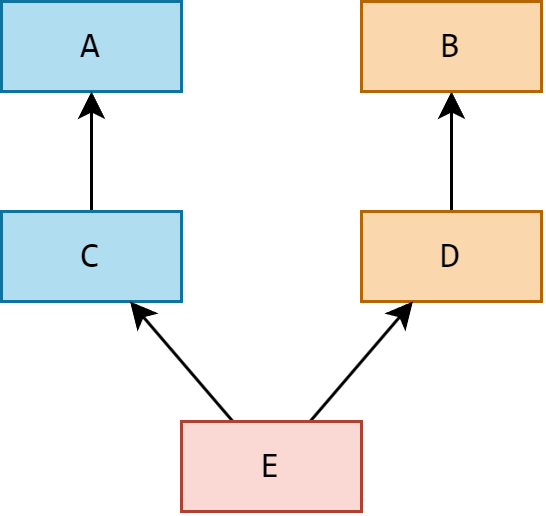
\includegraphics[width=.36\textwidth]{../images/generalized_parts/10_multiple_inheritance_example.png}
    \caption{多重继承关系示例}
\end{figure}
那么它的运行结果将是怎样的呢?\\\noindent\rule{\linewidth}{.2pt}\texttt{
A::A()\\
C::C()\\
B::B()\\
D::D()\\
E::E()
}\\\noindent\rule{\linewidth}{.2pt}
运行过程中总共有五个输出,我们可以把它分成三个过程:
\begin{enumerate}
    \item 调用 \lstinline@C@ 的构造函数。在这一过程中,\lstinline@A::A()@ 先调用,然后是 \lstinline@C::C()@。虽然在 \lstinline@E::E()@ 当中我们把 \lstinline@D{}@ 写在了 \lstinline@C{}@ 前面,但是这并不会改变构造函数调用的顺序——这个顺序是取决于继承顺序的。
    \item 调用 \lstinline@D@ 的构造函数。在这一过程中,\lstinline@B::B()@ 先调用,然后是 \lstinline@D::D()@。
    \item 完成了 \lstinline@C::C()@ 和 \lstinline@D::D()@ 的调用之后,\lstinline@E::E()@ 调用。
\end{enumerate}
不要觉得多重继承中的初始化顺序很复杂,其实只是多了一项准则而已:按多重继承的基类顺序调用各个基类的构造函数——简单点说,从左到右。对于这个继承顺序来说,调用 \lstinline@E::E()@ 之前就应当先后调用 \lstinline@C::C()@ 和 \lstinline@D::D()@。至于这两个构造函数要干什么,那不是 \lstinline@E@ 应当管的事情。从运行结果上看,\lstinline@C::C()@ 在 \lstinline@D::D()@ 之前,\lstinline@D::D()@ 又在 \lstinline@E::E()@ 这前,这就够了。\par
\subsection*{菱形继承结构的重复成员}
我们说,派生类的对象相当于内嵌了一个基类的对象;或者说,派生类相当于拥有基类的成员\footnote{即便基类的私有成员对派生类不可见。}。多重继承会为我们带来另一个棘手的问题,就是在菱形的继承关系下,公共基类的对象,或者说成员,发生了重复。\par
\begin{lstlisting}
struct Base { int num {0}; }; //Base类中有num成员
struct A : Base {}; //A类有继承自Base的num成员
struct B : Base {}; //B类有继承自Base的num成员
struct Derived : A, B {}; //Derived会继承A和B类的num成员各一个
int main() {
    Derived de;
    std::cout << &de.A::num << std::endl << &de.B::num;
    //de的A::num成员和B::num成员是同一成员吗?地址值能告诉我们答案
}
\end{lstlisting}
这段代码的运行结果是\\\noindent\rule{\linewidth}{.2pt}\texttt{
0x7ffc1fc88548\\
0x7ffc1fc8854c
}\\\noindent\rule{\linewidth}{.2pt}
换句话说,虽然 \lstinline@Derived@ 从根本上来说继承自 \lstinline@Base@,但是因为多重继承的缘故,它实际上有了两份 \lstinline@Base::num@ 成员,一个来自基类 \lstinline@A@,另一个来自基类 \lstinline@B@。\par
\begin{figure}[htbp]
    \centering
    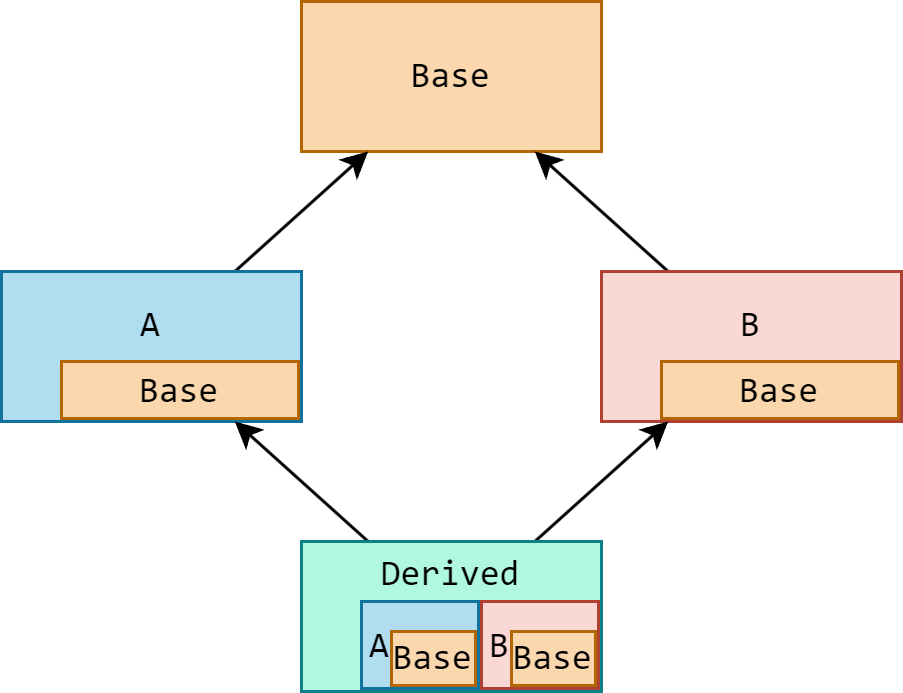
\includegraphics[width=.56\textwidth]{../images/generalized_parts/10_diamond_inheritance.png}
    \caption{菱形继承关系下,\lstinline@Derived@ 类内嵌了两份 \lstinline@Base@ 类对象}
\end{figure}
在多数情况下,这并不是我们想要的结果,而且还会引发无数的麻烦——比如说,内存空间的浪费,我们明明只需要一份数据,但多重继承为我们搞出了两份数据;再比如说,名称的歧义和冲突,我们不能单纯写成 \lstinline@d.num@,必须写成 \lstinline@d.A::num@ 或 \lstinline@d.B::num@。它们本应该相同的。而在C++中,解决这个问题的对策,就是下一节中要讲到的虚继承。\par
